%% main.tex — International Journal of Data Science and Analytics submission
%% "From Contemporaneous to Prospective: Quantifying Target Leakage in
%%  Student Academic Risk Prediction with Lightweight Temporal Models"
%%
%% All experimental numbers are injected from results/*.json via numbers.tex
%% (regenerate with: python3 experiments/build_paper_artifacts.py). No number in
%% this file is hard-coded.

\documentclass[sn-mathphys,Numbered]{sn-jnl}

\usepackage{graphicx}
\usepackage{multirow}
\usepackage{manyfoot}
\usepackage{amsmath,amssymb,amsfonts}
\usepackage{amsthm}
\usepackage[title]{appendix}
\usepackage{xcolor}
\usepackage{booktabs}
\usepackage{longtable}
\usepackage{array}
\usepackage{tikz}
\usetikzlibrary{positioning,calc,arrows,decorations.pathreplacing}
\usepackage{hyperref}

\raggedbottom

\begin{document}

\title[From Contemporaneous to Prospective in Academic Risk Prediction]{From Contemporaneous to Prospective: Quantifying Outcome-Window Inflation in Student Academic Risk Prediction with Lightweight Temporal Models}

\author[1]{\fnm{Jinyun} \sur{Hu}}\email{hujinyun1216@126.com}
\author[2]{\fnm{Xuenan} \sur{Du}}\email{1032950096@qq.com}
\author[2]{\fnm{Wen} \sur{Song}}\email{845540559@qq.com}
\author[3]{\fnm{Jian} \sur{Su}}\email{sujian328@163.com}
\author[2]{\fnm{Na} \sur{Li}}\email{389859429@qq.com}
\author[4]{\fnm{Jiangbo} \sur{Guo}}\email{jiangboguo79@163.com}
\author*[3]{\fnm{Huayan} \sur{Shang}}\email{Shyshy1981@126.com}

\affil[1]{\orgdiv{School of Digital Finance and Management}, \orgname{Dongying Vocational College}, \city{Dongying}, \postcode{257091}, \country{China}}
\affil[2]{\orgdiv{School of Cultural Tourism, Health Care and Education}, \orgname{Dongying Vocational College}, \city{Dongying}, \postcode{257091}, \country{China}}
\affil[3]{\orgdiv{School of Public Education}, \orgname{Dongying Vocational College}, \city{Dongying}, \postcode{257091}, \country{China}}
\affil[4]{\orgname{Dongying Vocational College}, \city{Dongying}, \postcode{257091}, \country{China}}

%% AUTO-GENERATED by experiments/build_paper_artifacts.py — do not edit by hand.
\newcommand{\nOULADenrol}{32\,593}
\newcommand{\nOULADstudents}{28\,785}
\newcommand{\nEdNetusers}{24\,736}
\newcommand{\nEdNetBins}{10}
\newcommand{\ouladLzero}{9.3\%}
\newcommand{\ednetLzero}{3.1\%}
\newcommand{\ouladLone}{37.9\%}
\newcommand{\ednetLone}{23.3\%}
\newcommand{\ouladLtwo}{21.6\%}
\newcommand{\ednetLtwo}{42.5\%}
\newcommand{\ouladLthree}{31.2\%}
\newcommand{\ednetLthree}{31.0\%}
\newcommand{\bilstmParams}{70\,948}
\newcommand{\gapOULADaccRange}{9.1--12.9}
\newcommand{\gapOULADqwkRange}{0.16--0.25}
\newcommand{\gapOULADqwkMax}{0.25}
\newcommand{\gapEdNetaccRange}{39.3--46.6}
\newcommand{\gapEdNetqwkRange}{0.50--0.58}
\newcommand{\gapEdNetqwkMax}{0.58}
\newcommand{\ouladProXGBFone}{0.527}
\newcommand{\ouladProXGBqwk}{0.667}
\newcommand{\ouladProBiLSTMFone}{0.553}
\newcommand{\ouladProLSTMFone}{0.552}
\newcommand{\ouladProLSTMqwk}{0.685}
\newcommand{\ednetProLSTMFone}{0.465}
\newcommand{\ouladProXGBoff}{92.2\%}
\newcommand{\ouladProXGBsev}{12.4\%}
\newcommand{\ouladProXGBsevover}{2.7\%}
\newcommand{\ednetBestSummary}{Gradient Boosting macro-F1 $0.459$, QWK $0.501$}
\newcommand{\ednetProBiLSTMFone}{0.457}
\newcommand{\ednetProBestoff}{95.6\%}
\newcommand{\ednetProBestsev}{0.7\%}
\newcommand{\ednetProBestsevover}{14.6\%}
\newcommand{\ednetProLSTMsev}{18.0\%}
\newcommand{\ednetProLSTMsevover}{8.9\%}
\newcommand{\pOULADfam}{0.001}
\newcommand{\pEdNetfam}{0.596}
\newcommand{\tempGapAccRange}{7.7--15.9}
\newcommand{\tempGapQwkRange}{0.14--0.18}
\newcommand{\tempProsAccXGB}{0.573}
\newcommand{\tempProsQwkLSTM}{0.667}
\newcommand{\ednetDoseXGBAcc}{0.786}
\newcommand{\ednetDoseBiAcc}{0.982}
\newcommand{\assistAccFirst}{0.414}
\newcommand{\assistAccLast}{0.701}
\newcommand{\assistQwkFirst}{0.437}
\newcommand{\assistQwkLast}{0.770}
\newcommand{\assistCohort}{2{,}314}
\newcommand{\matchedExtAcc}{7.0}
\newcommand{\matchedLeakAcc}{0.6}
\newcommand{\matchedExtQwk}{0.13}
\newcommand{\matchedLeakQwk}{0.00}
\newcommand{\matchedLeakAccBi}{1.7}
\newcommand{\matchedExtAccBi}{10.7}
\newcommand{\matchedExtQwkBi}{0.17}
\newcommand{\matchedLeakEarlyMax}{1.7}
\newcommand{\matchedLeakLateMax}{1.7}
\newcommand{\gapCIOULAD}{$+4.6$\,pp [$3.1$, $6.1$]}
\newcommand{\gapCIEdNet}{$+13.9$\,pp [$10.1$, $17.8$]}
\newcommand{\tunedOULADmodel}{BiLSTM-Attention}
\newcommand{\tunedOULADFone}{0.560}
\newcommand{\tunedOULADqwk}{0.685}
\newcommand{\aprioriOULADFone}{0.553}
\newcommand{\aprioriOULADqwk}{0.675}
\newcommand{\tunedEdNetmodel}{BiLSTM-Attention}
\newcommand{\tunedEdNetFone}{0.466}
\newcommand{\tunedEdNetqwk}{0.433}
\newcommand{\aprioriEdNetFone}{0.457}
\newcommand{\aprioriEdNetqwk}{0.416}
\newcommand{\doseXGBaccFirst}{0.614}
\newcommand{\doseXGBaccLast}{0.699}
\newcommand{\doseXGBqwkFirst}{0.667}
\newcommand{\doseXGBqwkLast}{0.809}
\newcommand{\doseXGBmonotoneAcc}{monotonically}
\newcommand{\doseLSTMaccFirst}{0.567}
\newcommand{\doseLSTMaccLast}{0.692}
\newcommand{\doseLSTMqwkFirst}{0.685}
\newcommand{\doseLSTMqwkLast}{0.843}
\newcommand{\doseLSTMmonotoneAcc}{monotonically}
\newcommand{\ordAccRange}{9.3--16.1}
\newcommand{\ordQwkRange}{0.19--0.24}


\abstract{Predictive models of student academic risk are frequently evaluated on formulations in which the predictors cover the same period as the outcome; the reported accuracy then partly reflects label reconstruction rather than forecasting ability. We quantify that inflation and demonstrate the corrective protocol. We contrast \emph{contemporaneous} formulations, in which predictors may include the label-defining signals, with \emph{prospective} formulations in which prediction precedes the labelled period (the $X_t \rightarrow Y_{t+1}$ requirement). On two public benchmarks --- the Open University Learning Analytics Dataset (\nOULADenrol{} enrolments by \nOULADstudents{} students) and EdNet-KT1 (\nEdNetusers{} users) --- we evaluate six models, from logistic regression to an attention-augmented bidirectional long short-term memory (LSTM; \bilstmParams{} parameters), under identical student-level splits, training-only preprocessing, and an ordinal evaluation protocol (macro-F1, mean absolute error, weighted $\kappa$, severe-underestimation rate) with student-level bootstrap confidence intervals. Contemporaneous formulations inflate accuracy by \gapOULADaccRange{} points on OULAD and \gapEdNetaccRange{} points on EdNet-KT1, and weighted $\kappa$ by up to \gapOULADqwkMax{} and \gapEdNetqwkMax{} --- exceeding the spread between competing model families. A matched-window control decomposes the effect: on OULAD it is dominated by legitimate later information, on EdNet-KT1 it is almost entirely label reconstruction, and the dose--response replicates on a third platform. Under the prospective protocol the lightweight temporal models are competitive with tree ensembles but do not dominate them; we report model rankings rather than a best-everywhere claim, and release a multi-source fusion pipeline with scripts that reproduce every number. Academic risk prediction should therefore be specified and reported prospectively.}

\keywords{Academic risk prediction, Target leakage, Learning analytics, Ordinal classification, Prospective evaluation, Educational data science}

\maketitle

%% =========================================================
\section{Introduction}\label{sec:intro}

Educational institutions increasingly operate a portfolio of disconnected information systems: academic management systems holding grades and credit records, learning-management systems recording online interaction, student-affairs systems covering demographics and attendance and --- in vocational settings under industry--university integration policies --- cooperation platforms that carry workplace-learning signals such as internships, enterprise supervisor ratings, and skill certifications \cite{Daniel2015,Ferguson2012,Liu2023}. Fusing these heterogeneous sources into a form suitable for predictive modelling is a data-engineering problem in its own right \cite{Gasevic2015}, and a substantial literature now reports machine-learning models that identify struggling students from such fused data with high reported accuracy \cite{Romero2020,Hellas2018,ZawackiRichter2019}.

A large share of those reports share a quiet methodological weakness. The outcome to be predicted --- a semester grade, a warning level, a dropout decision --- is defined by variables (grades, failure counts, engagement totals) that are themselves available at the end of the period being labelled. When the feature window extends over the same period as the label, the ``prediction'' task is partly or wholly \emph{label reconstruction}: the model recovers the deterministic rule that produced the label. This is the target-leakage problem familiar from applied data-mining practice \cite{Kaufman2012,Kapoor2023}, and it has been documented specifically in learning-analytics evaluation practice \cite{Hellas2018,Whitehill2015}. Yet because each published study reports a single number under a single formulation, the field has no shared sense of \emph{how large} the inflation is when the same model family, split, and target are moved from a contemporaneous to a strictly prospective formulation.

This paper measures that gap and demonstrates the corrective protocol. Our interest grew out of a multi-source early-warning deployment at a Chinese vocational college, where a four-level warning rule is defined operationally from semester GPA, failed-course counts, and attendance. Specifying a strictly prospective version of that task --- predicting the \emph{next} period's warning level from information available \emph{before} the period begins --- proved to be a fundamentally different modelling problem than the contemporaneous classification the operational rule suggests, and the public-benchmark experiments reported here were designed to quantify the difference in a setting that other researchers can reproduce exactly. The institutional system itself is used in this paper only as a design context and software case study; no institutional performance figures are reported, because the underlying records cannot be released or independently audited.

We pose three research questions.
\textbf{(RQ1)} How much does measured performance change when the information boundary moves from prospective to contemporaneous, under matched targets, splits, and protocol?
\textbf{(RQ2)} How does this formulation effect vary across model families and across the two benchmarks?
\textbf{(RQ3)} How much of the effect is legitimate information accumulation, and how much is label-defining contamination?

To answer these questions we run a controlled comparison on two large public educational datasets with complementary structure: the Open University Learning Analytics Dataset (OULAD) \cite{Kuzilek2017}, in which the outcome is a course-level result and the predictor window is the first 30\,\% of the course; and EdNet-KT1 \cite{Choi2020}, in which the outcome is derived from the second half of each learner's practice sequence and predictors come from the first half. Six models --- logistic regression, random forest, gradient boosting, XGBoost, LSTM, and a lightweight BiLSTM with additive attention --- are trained under an identical protocol: student-level (user-level) splits that never place one learner in two splits, preprocessing fitted on training data only, no test-informed tuning, and an ordinal metric suite with student-level bootstrap confidence intervals. The same experiment is repeated in a contemporaneous regime in which the label-defining signals are deliberately included in the feature window, yielding a direct, per-model measurement of leakage inflation.

The study makes the following contributions:
\begin{enumerate}
  \item \textbf{A controlled quantification of the formulation effect.} Across two public benchmarks (\nOULADenrol{} OULAD enrolments; \nEdNetusers{} EdNet-KT1 users) and six model families we measure the contemporaneous-versus-prospective gap --- \gapOULADaccRange{} and \gapEdNetaccRange{} accuracy points, weighted $\kappa$ up to \gapOULADqwkMax{} and \gapEdNetqwkMax{} --- under identical targets, splits, and protocol. The total effect exceeds the spread between competing architectures.
  \item \textbf{A decomposition of the effect.} A matched-window control and a graded dose--response analysis separate legitimate information accumulation from label-defining contamination: on OULAD the effect is dominated by the former (window extension adds \matchedExtAcc{} to \matchedExtAccBi{} points; injecting the final-exam score adds at most \matchedLeakLateMax{}), whereas on EdNet-KT1, whose outcome is a deterministic function of the labelled sequence, the effect is essentially label reconstruction.
  \item \textbf{A decision-time-aligned evaluation protocol.} Student-level splits, strictly availability-filtered features, training-only preprocessing, single-shot test evaluation, an ordinal metric suite with student-level bootstrap intervals, and a released end-to-end pipeline whose tensor layer enforces the cut structurally.
\end{enumerate}
The multi-source fusion pipeline of Section~\ref{sec:pipeline} and the attribution analyses of Section~\ref{sec:res_shap} support these contributions --- as released software and as secondary evidence respectively --- rather than being contributions in their own right.

\medskip
The remainder of the paper is organised as follows. Section~\ref{sec:related} reviews related work on academic risk prediction, target leakage, and temporal models for learning data. Section~\ref{sec:formulation} formalises the contemporaneous/prospective contrast and the ordinal targets. Section~\ref{sec:data} describes the fusion pipeline and the two benchmarks. Section~\ref{sec:method} specifies the evaluation protocol, models, and metrics. Section~\ref{sec:results} reports results. Section~\ref{sec:discussion} discusses implications, including qualitative lessons from the institutional deployment, and Section~\ref{sec:limitations} states limitations. Section~\ref{sec:conclusion} concludes.

%% =========================================================
\section{Related Work}\label{sec:related}

\subsection{Academic Risk Prediction and Reported Accuracy}\label{sec:rw_risk}

Predicting academic outcomes is one of the most active areas of educational data mining and learning analytics \cite{Romero2020,ZawackiRichter2019}. Deployed early-warning practice has largely relied on cumulative indicators such as GPA thresholds and failure counts \cite{Jayaprakash2014,Marbouti2016}, and the research literature reports logistic regression \cite{Costa2017}, random forests \cite{Breiman2001,MarquezVera2016}, gradient-boosted trees \cite{Chen2016}, and ensemble or deep approaches \cite{Amrieh2016,Waheed2024} for at-risk identification. Systematic reviews repeatedly observe that evaluation practice varies widely and that reported accuracies are often optimistic \cite{Hellas2018,Whitehill2015}: outcome-contemporaneous signals appear among predictors, samples are small, and validation is frequently internal and random. Recent work continues to report strong results from clickstream and log data \cite{Pecuchova2024,Vaarma2024,Marcolino2025,Mustofa2025,Qiu2022,Wang2021}, typically without separating the contribution of the modelling from the contribution of the feature window. What is missing --- and what this paper provides --- is a controlled measurement of how much the formulation itself contributes to the reported number.

\subsection{Target Leakage in Applied Machine Learning}\label{sec:rw_leakage}

Leakage --- the presence of information in training data that will not be available at prediction time --- has long been identified as a central failure mode of applied data mining \cite{Kaufman2012}. Kapoor and Narayanan \cite{Kapoor2023} document its pervasiveness across machine-learning-based science and trace its consequences for reproducibility. In learning analytics specifically, Hellas et al. \cite{Hellas2018} and Whitehill \cite{Whitehill2015} discuss post-outcome signals contaminating predictors. Two remedies recur in the literature: restricting features to a pre-outcome window, and temporal or group-aware validation. Both cost apparent accuracy, and papers that adopt them tend to report lower numbers than papers that do not --- a dynamic that rewards the leakage-prone practice. Closest in spirit to our setting, the CAPIRE framework \cite{Paz2025} builds a leakage-aware data layer into curriculum-aware student-trajectory analytics --- a safeguard-oriented contribution. What this line of work has not yet provided for academic risk prediction is a measurement of the incentive itself, and our contribution is not a new detector but exactly that: a measured, model-by-model account of how many points of accuracy and $\kappa$ the leaky formulation buys.

\subsection{Temporal Deep Learning for Learning-Process Data}\label{sec:rw_temporal}

Learning-process data are naturally sequential, and recurrent architectures have been applied to MOOC dropout \cite{Fei2015}, knowledge tracing \cite{Piech2015}, completion forecasting \cite{Wang2021}, and e-learning behaviour analytics \cite{Qiu2022}. Bidirectional LSTMs \cite{Graves2005,Hochreiter1997} integrate context from both directions of the observation window, and additive attention \cite{Bahdanau2015,Vaswani2017} provides data-driven time-step weights with a degree of temporal interpretability. Heterogeneous extensions model student trajectories as richer structures \cite{Cheng2024}. A recurrent finding in benchmark studies is that the advantage of deep temporal models over tuned tree ensembles is small once feature sets are matched \cite{Waheed2024,Yin2024}; our protocol makes this comparison explicit by appending the identical static covariates to the flat and temporal inputs, so that any measured difference is attributable to temporal structure rather than to feature access.

\subsection{Evaluation Practice: Ordinal Targets, Grouped Resampling, Attribution}\label{sec:rw_eval}

Graduated warning schemes support differentiated intervention \cite{Arnold2012,Pistolesi2017} but turn the target into an ordered variable; treating the levels as nominal discards the severity structure of errors, which is precisely what matters operationally when a severely at-risk student is labelled low-risk. Ordinal agreement measures such as quadratic weighted $\kappa$ \cite{Cohen1960,Landis1977} and distance-based error rates address this. On the resampling side, repeated observations of the same student violate the independence assumptions of both random splits and observation-level bootstrap; group-aware splitting and student-level resampling are the corresponding corrections. Finally, SHAP attribution \cite{Lundberg2017} is increasingly used in educational models \cite{Marcolino2025,Mustofa2025}; attribution explains a model's output, not the causal process generating the data, and we position it accordingly.

%% =========================================================
\section{Problem Formulation}\label{sec:formulation}

\subsection{Contemporaneous versus Prospective Formulations}\label{sec:form_prospective}

Let $i$ index the unit of prediction --- a course enrolment (OULAD) or a learner (EdNet-KT1) --- and let $W_i$ denote the observation period over which longitudinal activity is recorded. The outcome $Y_i \in \{0,1,2,3\}$ is an ordered severity label determined by events across $W_i$ (Section~\ref{sec:form_labels}). A \emph{feature window} $[0, \tau_i] \subseteq W_i$ determines the information set
\begin{equation}
  \mathbf{X}_i(\tau_i) \;=\; \{\,\text{static attributes of } i\,\} \;\cup\; \{\,\text{activity signals of } i \text{ over } [0, \tau_i]\,\}.
\end{equation}

Two formulations of the prediction task are possible, and everything in this paper follows from the difference between them (Fig.~\ref{fig:conceptual}).

\begin{figure}[ht]
  \centering
  \resizebox{\textwidth}{!}{\definecolor{cblue}{HTML}{2A78D6}
\definecolor{corange}{HTML}{E8760E}
\definecolor{credark}{HTML}{9A3B1E}
\definecolor{cgray}{HTML}{8B8A80}
\definecolor{cpast}{HTML}{DCE9FA}
\definecolor{cfut}{HTML}{EDEDEA}
\begin{tikzpicture}[
  font=\scriptsize,
  lab/.style={font=\tiny\bfseries, text=black!45},
  tlab/.style={font=\tiny, text=black!60},
  ann/.style={font=\tiny, text=black!55, align=center},
]
% panel (a)
\node[anchor=west, font=\scriptsize\bfseries] at (0, 8.85) {(a)~The prediction task: predict the outcome from earlier information};
\draw[->, line width=0.9pt, black!60] (0.3, 7.3) -- (15.2, 7.3);
\node[tlab, anchor=north] at (0.3, 7.18)  {course / sequence start};
\node[tlab, anchor=north] at (10.8, 7.18) {decision time $\tau$};
\node[tlab, anchor=north] at (15.1, 7.18) {outcome};
\draw[black!60, line width=1.2pt] (10.8, 6.95) -- (10.8, 7.65);
\foreach \x/\l in {2.2/engagement, 5.2/assessments, 8.4/coursework}{
  \fill[cblue] (\x, 7.3) circle (0.075);
  \node[tlab, yshift=5pt] at (\x, 7.3) {\l};
}
\fill[credark] (14.0, 7.3) circle (0.075);
\node[tlab, yshift=5pt, text=credark] at (14.0, 7.3) {grades · failure · withdrawal};
\draw[decorate, decoration={brace, amplitude=4pt}, black!45] (0.4, 7.95) -- (10.7, 7.95);
\node[lab, text=cblue!60!black] at (5.55, 8.32) {information available at the decision time};
\draw[decorate, decoration={brace, amplitude=4pt}, black!45] (10.9, 7.95) -- (15.1, 7.95);
\node[lab, text=credark] at (13.0, 8.32) {label-defining region};
% panel (b)
\node[anchor=west, font=\scriptsize\bfseries] at (0, 5.55) {(b)~Prospective: decision-time aligned};
\fill[cpast]  (0.4, 3.6) rectangle (10.7, 4.9);
\fill[cfut]   (10.8, 3.6) rectangle (15.1, 4.9);
\draw[black!50, line width=0.5pt]  (0.4, 3.6) rectangle (10.7, 4.9);
\draw[black!50, line width=0.5pt]  (10.8, 3.6) rectangle (15.1, 4.9);
\node[font=\tiny, text=cblue!50!black] at (5.5, 4.45) {predictors: everything observed before $\tau$};
\node[font=\tiny, text=black!55] at (12.9, 4.45) {outcome $Y$};
\node[font=\tiny, text=black!45] at (12.9, 4.05) {observed only at the end};
\draw[black!60, line width=1.2pt] (10.8, 3.35) -- (10.8, 5.15);
\node[tlab, anchor=east] at (10.68, 3.5) {$\tau$};
\draw[->, line width=0.8pt, cblue] (5.5, 3.32) .. controls (8.6, 2.7) .. (12.6, 3.42);
\node[font=\tiny, text=cblue!50!black] at (7.6, 2.72) {prediction made at $\tau$, before the outcome exists};
% panel (c)
\node[anchor=west, font=\scriptsize\bfseries] at (0, 1.85) {(c)~Contemporaneous: outcome-overlapping};
\fill[cpast]   (0.4, -0.1) rectangle (8.9, 1.2);
\fill[corange!22] (8.9, -0.1) rectangle (15.1, 1.2);
\fill[corange!45] (11.6, -0.1) rectangle (15.1, 1.2);
\draw[black!50, line width=0.5pt]  (0.4, -0.1) rectangle (15.1, 1.2);
\node[font=\tiny, text=cblue!50!black] at (4.6, 0.75) {predictors: everything observed before $\tau$};
\node[font=\tiny, text=credark] at (13.35, 0.75) {+ label-defining signals};
\node[font=\tiny, text=black!55] at (10.2, 0.32) {later information,};
\node[font=\tiny, text=black!55] at (10.2, -0.02) {legitimately acquired};
\node[font=\tiny, text=credark] at (13.9, 0.32) {outcome-determining};
\draw[black!60, line width=1.2pt] (10.8, -0.35) -- (10.8, 1.45);
\node[tlab, anchor=east] at (10.68, -0.2) {$\tau$};
% panel (d)
\node[anchor=west, font=\scriptsize\bfseries] at (0, -1.35) {(d)~Same task, same model, same split --- only the information boundary moves};
\node[font=\tiny, text=black!60] at (7.7, -1.95) {what the added window contains};
\draw[->, line width=0.8pt, black!55] (6.6, -2.12) -- (3.6, -2.62);
\draw[->, line width=0.8pt, black!55] (8.8, -2.12) -- (11.8, -2.62);
\draw[cblue, line width=0.6pt, rounded corners=3pt, fill=cblue!8] (0.8, -2.75) rectangle (6.0, -3.95);
\node[font=\tiny, text=cblue!50!black, align=center] at (3.4, -3.35) {legitimate temporal accumulation\\[-2pt]{\tiny (OULAD: the window extension adds $+7.0$ to $+10.7$\,pp)}};
\draw[credark, line width=0.6pt, rounded corners=3pt, fill=credark!6] (9.4, -2.75) rectangle (14.9, -3.95);
\node[font=\tiny, text=credark, align=center] at (12.15, -3.35) {label reconstruction\\[-2pt]{\tiny (EdNet-KT1: injection of the outcome-determining sequence adds up to $+46.6$\,pp)}};
\node[font=\scriptsize] at (7.7, -4.55) {$\Delta_{\mathrm{formulation}} \;=\; \mathrm{Performance}_{\mathrm{contemporaneous}} \; - \; \mathrm{Performance}_{\mathrm{prospective}}$};
\node[font=\tiny, text=black!50] at (7.7, -5.05) {same model · same target · same split · same protocol --- only the boundary moves};
\end{tikzpicture}
}
  \caption{Information-window formulation of academic-risk prediction. (a)~The prediction task: the outcome is determined at the end of a period, while a warning system must act at a decision time $\tau$ inside it. (b)~The prospective formulation restricts predictors to the decision-time window. (c)~The contemporaneous formulation extends predictors over the labelled period; the added window contains both legitimately later information and, at its end, the label-defining signals. (d)~The formulation effect $\Delta_{\mathrm{formulation}}$ is measured under identical models, targets, splits, and protocol, and decomposes into the two regimes that Sections~\ref{sec:res_decompose} and~\ref{sec:res_dose} quantify.}
  \label{fig:conceptual}
\end{figure}

\textbf{Contemporaneous.} $\tau_i = |W_i|$: the feature window covers the whole labelled period, so $\mathbf{X}_i(\tau_i)$ may contain the label-defining signals themselves. The task is
\begin{equation}
  \mathbf{X}_i(|W_i|) \;\longrightarrow\; Y_i,
\end{equation}
and the achievable performance is bounded by how much of $Y_i$ is a deterministic function of $\mathbf{X}_i(|W_i|)$. We call this regime \emph{contemporaneous} and treat it as a label-reconstruction reference: models operating in it partially re-derive the labelling rule rather than forecast an unseen outcome \cite{Kaufman2012}.

\textbf{Prospective.} $\tau_i < |W_i|$: prediction happens at a cut-off strictly inside the period, using only information then available:
\begin{equation}
  \mathbf{X}_i(\tau_i) \;\longrightarrow\; Y_i, \qquad \tau_i = \lceil p \, |W_i| \rceil,\; p \in (0,1).
\end{equation}
This is the operational form of early warning --- acting before the outcome exists --- and is the analogue, for period-labelled data, of the standard $X_t \rightarrow Y_{t+1}$ requirement in longitudinal risk prediction. We use $p = 0.30$ for OULAD (first 30\,\% of each course presentation) and $p = 0.50$ for EdNet-KT1 (first half of each learner's sequence).

The quantification target of this paper is the per-model gap between the two regimes:
\begin{equation}
  \Delta_M \;=\; \mathrm{score}\big(M, \text{contemporaneous}\big) - \mathrm{score}\big(M, \text{prospective}\big),
\end{equation}
for every model $M$ and score in our metric suite. Any $\Delta_M > 0$ measures the total formulation effect: the combined advantage of information that legitimately arrives later in the period and of the label-defining signals that only exist once the outcome does. Section~\ref{sec:res_decompose} separates the two components with a matched-window control, and the dose--response analysis of Section~\ref{sec:res_dose} traces their continuous version.

\subsection{Hierarchical Ordinal Targets}\label{sec:form_labels}

Both benchmarks require mapping a native outcome to a four-level ordered severity scale, consistent with graduated warning schemes in institutional practice \cite{Arnold2012,Pistolesi2017}. Table~\ref{tab:labels} states the mappings used throughout; they are identical across the two regimes, so no difference between regimes can be attributed to the labelling.

\begin{table}[ht]
\caption{Ordinal label definitions. Levels are ordered by increasing severity; the same mapping is applied in both regimes.\label{tab:labels}}
\begin{tabular*}{\textwidth}{@{\extracolsep\fill}llp{8.2cm}}
\toprule
\textbf{Dataset} & \textbf{Level} & \textbf{Definition (outcome observed at the end of the labelled period)} \\
\midrule
\multirow{4}{*}{OULAD}
 & 0 & \textit{Distinction} --- final result ``Distinction'' \\
 & 1 & \textit{Pass} --- final result ``Pass'' \\
 & 2 & \textit{Fail} --- final result ``Fail'' \\
 & 3 & \textit{Withdrawn} --- final result ``Withdrawn'' \\
\midrule
\multirow{4}{*}{EdNet-KT1}
 & 0 & second-half mean correctness $\geq 0.85$ \\
 & 1 & $0.70 \leq$ mean correctness $< 0.85$ \\
 & 2 & $0.50 \leq$ mean correctness $< 0.70$ \\
 & 3 & mean correctness $< 0.50$ \\
\bottomrule
\end{tabular*}
\footnotetext{The OULAD mapping treats withdrawal as the most severe level, reflecting loss of enrolment rather than graded failure; Section~\ref{sec:limitations} discusses the sensitivity of conclusions to this choice.}
\end{table}

For OULAD we treat withdrawal as the most severe level because, from a warning system's perspective, the loss of enrolment ends the possibility of instructional support and is the operationally most consequential outcome; graded failure is ordered between pass and withdrawal. This choice is a modelling convention rather than a ground truth, and Section~\ref{sec:limitations} reports a full re-run under the alternative ordering (graded failure most severe) showing that the formulation effect is unchanged. Because levels are ordered, we treat all error as ordinal distance: confusing adjacent levels is a lesser error than crossing multiple levels, and labelling a level-3 (most severe) case as level 0--1 is the costliest mistake a warning system can make.

\subsection{Units, Splits, and Resampling}\label{sec:form_units}

The prediction unit is the enrolment (OULAD) or learner (EdNet-KT1); the \emph{resampling and splitting unit} is the student. OULAD contains \nOULADenrol{} enrolments contributed by only \nOULADstudents{} distinct students, so an observation-level split places most multi-course students in both training and test data; we therefore split at the student level (70/15/15, stratified by the student's most severe observed label). EdNet-KT1 contributes one sequence per user, so its user-level split is student-level by construction. All confidence intervals are produced by resampling \emph{students} with replacement and pooling all their observations, which preserves the within-student dependence that observation-level bootstrap destroys.

%% =========================================================
\section{Data and Fusion Pipeline}\label{sec:data}

\subsection{A Multi-Source Fusion Pipeline as Reusable Software}\label{sec:pipeline}

The study is motivated by a multi-source institutional context: a Chinese vocational college operating four independent systems --- academic management (grades, credits), a learning platform (interaction traces), student affairs (demographics, attendance), and an industry--university cooperation platform (internships, supervisor evaluations, skill certifications) \cite{Liu2023}. Fusing such sources for any predictive purpose requires an integration layer, and integrating them \emph{safely} --- without letting the label-defining operational variables leak into the predictor window --- requires that the integration layer expose the temporal cut explicitly.

The pipeline released with this paper (Fig.~\ref{fig:pipeline}) follows the extractor$\,\to\,$merge$\,\to\,$tensor$\,\to\,$manifest pattern we use in the institutional deployment: (i)~each source system is wrapped by an extractor exposing a tabular view keyed on (\texttt{student}, \texttt{period}); (ii)~views are merged partition-parallel on the key; (iii)~a tensor constructor emits $\mathbf{X} \in \mathbb{R}^{N \times T \times F}$ with an explicit mask of which periods are pre-cutoff; (iv)~a manifest gate makes each phase idempotent and failure-tolerant. The cut-off semantics of Section~\ref{sec:form_prospective} are enforced at the tensor-construction step: label-defining variables are written to a separate, post-cutoff table that downstream models cannot join into the training tensor. The pipeline ships with a synthetic-data generator preserving the institutional feature schema, so the full integration path can be exercised without access to protected records. We use this infrastructure as the case-study backbone of the paper; no institutional performance figures are reported or claimed.

\begin{figure}[ht]
  \centering
  \resizebox{0.88\textwidth}{!}{% Figure 1 — multi-source fusion pipeline with an explicit prospective cut.
% Inline TikZ (document-matched fonts); compiled inside main.tex via
%   \resizebox{\textwidth}{!}{\input{figures/fig1_architecture}}
\definecolor{pipeblue}{HTML}{2A78D6}
\definecolor{pipeviolet}{HTML}{4A3AA7}
\definecolor{pipered}{HTML}{C0392B}
\definecolor{winblue}{HTML}{DBE9FB}
\definecolor{winred}{HTML}{FADCDC}
\begin{tikzpicture}[
  >={stealth},
  box/.style={draw=black!42, line width=0.5pt, rounded corners=2.4pt, align=center,
              inner sep=3.0pt, font=\scriptsize, fill=white},
  src/.style={box, fill=black!4, font=\tiny, inner sep=2.4pt},
  stage/.style={font=\tiny\bfseries, text=black!45},
  ann/.style={font=\tiny, text=black!50, align=center},
  bluebox/.style={box, draw=pipeblue, fill=pipeblue!8, text=pipeblue!35!black,
                  font=\scriptsize\bfseries, align=center},
  redbox/.style={box, draw=pipered, fill=pipered!7, text=pipered!45!black,
                 font=\scriptsize\bfseries, align=center},
  viobox/.style={box, draw=pipeviolet, fill=pipeviolet!7, text=pipeviolet!40!black,
                 font=\scriptsize\bfseries, align=center},
  flow/.style={->, line width=0.7pt, draw=black!55},
  bflow/.style={flow, draw=pipeblue},
  rflow/.style={flow, draw=pipered, dash pattern=on 2.2pt off 1.6pt},
  vflow/.style={flow, draw=pipeviolet},
]
%
% ---- row 1: pipeline -------------------------------------------------------
\node[src] (ams) at (0.55, 0.50)  {AMS};
\node[src] (lms) at (1.75, 0.50)  {LMS};
\node[src] (sas) at (0.55, -0.36) {SAS};
\node[src] (iucp) at (1.75, -0.36){IUCP};
\node[stage] at (1.15, 1.16) {SOURCES};
\draw[black!40, line width=0.6pt] (2.42, 0.50) -- (2.42, -0.36);
%
\node[box, align=center] (ext) at (4.05, 0) {per-source extractors\\[-2pt]{\tiny key (\texttt{student}, \texttt{period})}};
\node[stage] at (4.05, 1.16) {EXTRACT};
%
\node[box, align=center, fill=pipeblue!6, draw=pipeblue] (mrg) at (6.35, 0) {partition-parallel\\ merge};
\node[stage] at (6.35, 1.16) {INTEGRATE};
\node[box, dashed, inner sep=2.2pt, font=\tiny] (man) at (6.35, -0.94) {manifest gate};
\draw[densely dotted, draw=black!40] (mrg.south) -- (man.north);
\node[ann] at (6.35, -1.44) {idempotent · failure-tolerant};
%
\node[box, align=center, fill=pipeblue!6, draw=pipeblue] (con) at (8.70, 0) {tensor\\ constructor};
\node[stage] at (8.70, 1.16) {CONSTRUCT};
%
\draw[flow] (2.98, 0.07) -- (2.42, 0.07);
%
\draw[flow] (ext.east) -- (mrg.west);
\draw[flow] (mrg.east) -- (con.west);
%
% fork: constructor -> X (blue) / Y (red)
\node[bluebox] (xt) at (10.75, 0.78)  {training tensor $\mathbf{X}(\tau)$\\[-2pt]{\tiny pre-cutoff signals only}};
\node[redbox]  (yt) at (10.75, -0.78) {outcome table $Y$\\[-2pt]{\tiny post-cutoff · label-defining}};
\draw[bflow] (con.east) -- ++(0.16,0) |- (xt.west);
\draw[rflow, solid] (con.east) -- ++(0.16,0) |- (yt.west);
%
% models + evaluation
\node[viobox] (mdl) at (13.90, 0.78)  {flat + temporal models\\[-2pt]{\tiny BiLSTM-Attention (71K)}};
\node[viobox] (evl) at (13.90, -0.78) {ordinal metrics +\\[-2pt]{\tiny student-level bootstrap}};
\draw[bflow] (xt.east) -- (mdl.west);
\draw[vflow] (mdl.south) -- (evl.north);
\draw[rflow] (yt.east) -- (evl.west);
\node[ann, text=pipered] at (12.85, -1.58) {joined at evaluation only};
%
% ---- the cut: one red line from the fork down into the timeline ------------
\draw[pipered, line width=1.1pt] (9.02, -1.30) -- (9.02, -2.50);
\node[font=\tiny\bfseries, text=pipered, anchor=south west] at (9.12, -2.42) {prospective cut $\tau$};
%
% ---- row 2: timeline -------------------------------------------------------
\fill[winblue, draw=pipeblue, line width=0.5pt]  (0.40, -3.52) rectangle (9.02, -2.86);
\fill[winred,  draw=pipered, line width=0.5pt] (9.02, -3.52) rectangle (15.30, -2.86);
\node[font=\scriptsize\bfseries, text=pipeblue!40!black] at (4.71, -3.12)
  {feature window $[0,\tau]$ $\rightarrow$ $\mathbf{X}(\tau)$};
\node[font=\scriptsize\bfseries, text=pipered!45!black] at (12.16, -3.12)
  {labelled period $(\tau,|W|]$ $\rightarrow$ $Y$};
\node[ann, text=pipeblue!45!black] at (4.71, -3.40) {activity signals · early assessments};
\node[ann, text=pipered!45!black] at (12.16, -3.40) {label-defining signals: grades · failures · attendance};
%
\foreach \x in {2.2, 4.2, 6.4}{
  \draw[pipeblue, line width=0.8pt, fill=white] (\x, -3.19) circle (0.07);
}
\draw[pipered, line width=0.8pt, fill=white] (13.6, -3.19) circle (0.07);
\node[ann, text=pipered!45!black] at (13.6, -2.74) {final exam};
\node[ann, text=pipeblue!45!black] at (4.71, -2.74) {model sees only this side};
\node[ann] at (0.40, -3.86) {$t=0$};
\node[ann] at (15.30, -3.86) {$t=|W|$};
\node[ann, text=pipered!45!black] at (12.16, -3.86) {joined only at evaluation};
%
\end{tikzpicture}
}
  \caption{The released fusion pipeline. Per-source extractors emit (\texttt{student}, \texttt{period})-keyed views; the partition-parallel merge, gated by an idempotent manifest, produces the unified table; the tensor constructor routes pre-cutoff signals into the training tensor $\mathbf{X}(\tau)$ while label-defining variables are routed to a post-cutoff outcome table that is joined only at evaluation time.}
  \label{fig:pipeline}
\end{figure}

\subsection{Public Benchmarks}\label{sec:benchmarks}

Experiments use two public datasets with complementary structure (Table~\ref{tab:datasets}); neither contains institutional workplace-learning signals, which is precisely why they can be released and reproduced.

\textbf{OULAD} \cite{Kuzilek2017} covers 22 course presentations with \nOULADenrol{} enrolments by \nOULADstudents{} students. Predictors comprise enrolment demographics and prior study indicators (gender, region, highest education, IMD band, age band, disability, previous attempts, studied credits), VLE interaction aggregates (total clicks, active days, mean and dispersion of daily clicks) over the feature window, and assessment scores due within the window. The prospective window is the first 30\,\% of each presentation; the contemporaneous window is the full presentation and additionally includes all assessment scores, among them the final exam whose score largely determines the label.

\textbf{EdNet-KT1} \cite{Choi2020} is a large-scale knowledge-tracing corpus of learner practice interactions. From a deterministic random sample (seed~42) of \nEdNetusers{} users with at least 20 interactions, each sequence is split in half: features from the first half (per-segment correctness rates, segment lengths, response times, and inter-response gaps binned into \nEdNetBins{} equal-count tokens, plus first-half aggregates), outcome from the second half via the mean-correctness thresholds of Table~\ref{tab:labels}. In the contemporaneous regime, features are computed over the full sequence --- which contains the responses whose correctness defines the label --- and the label is likewise derived from the full sequence. EdNet-KT1 and ASSISTments therefore play a specific role in the design: because their outcomes are deterministic functions of the labelled sequences, its contemporaneous regime is a \emph{reconstruction regime} --- an analytical upper bound on formulation inflation rather than a realistic prediction task (Section~\ref{sec:res_leakage}). A third platform, ASSISTments 2009--2010 \cite{Feng2009} (problem-attempt logs; students with at least twenty attempts; the same four-level correctness thresholds), replicates the dose--response analysis of Section~\ref{sec:res_dose} on an independent knowledge-tracing corpus.

\begin{table}[ht]
\caption{Benchmarks and regimes. Percentages are shares of the analysis sample.\label{tab:datasets}}
\begin{tabular*}{\textwidth}{@{\extracolsep\fill}llrrrr}
\toprule
 & & \multicolumn{4}{c}{\textbf{Label distribution (\%)}} \\
\cmidrule(l){3-6}
\textbf{Dataset} & \textbf{Units} & \textbf{Level 0} & \textbf{Level 1} & \textbf{Level 2} & \textbf{Level 3} \\
\midrule
OULAD (enrolments) & \nOULADenrol{} & \ouladLzero & \ouladLone & \ouladLtwo & \ouladLthree \\
EdNet-KT1 (users)  & \nEdNetusers{} & \ednetLzero & \ednetLone & \ednetLtwo & \ednetLthree \\
\bottomrule
\end{tabular*}
\footnotetext{OULAD: 32{,}593 enrolments by 28{,}785 students; prospective cut at the first 30\,\% of each course presentation. EdNet-KT1: deterministic sample of users with $\geq 20$ interactions; prospective cut at the midpoint of each sequence.}
\end{table}

%% =========================================================
\section{Methodology}\label{sec:method}

\subsection{Leakage-Controlled Evaluation Protocol}\label{sec:protocol}

The protocol is identical across datasets, regimes, and models:
\begin{enumerate}
  \item \textbf{Student-level splits.} 70/15/15 train/validation/test. For OULAD the split is over students, stratified by the student's most severe observed label; for EdNet-KT1 it is over users, stratified by label. No student (user) appears in more than one split.
  \item \textbf{Training-only preprocessing.} Imputation, one-hot encoding of categoricals, and standardisation are fitted on the training split and applied unchanged to validation and test. Class weights are inverse-frequency weights computed on the training split only.
  \item \textbf{No test-informed selection.} Flat-model hyperparameters are fixed a priori (Table~\ref{tab:hyperparams}); temporal models early-stop on validation macro-F1. The test split is scored exactly once per model.
  \item \textbf{Information-fair temporal inputs.} Temporal models receive the regime-matching activity sequence with the model's static feature vector appended to every time step, so flat and temporal models see the same information and differ only in whether sequential structure is modelled.
\end{enumerate}

\subsection{Models}\label{sec:models}

Six models span the complexity range of common practice: \textbf{multinomial logistic regression} (L2, $C{=}1.0$); \textbf{random forest} \cite{Breiman2001} (300 trees, max depth 15); \textbf{gradient boosting} (200 estimators, depth 3); \textbf{XGBoost} \cite{Chen2016} (300 estimators, depth 6, lr 0.1); \textbf{LSTM} \cite{Hochreiter1997} (unidirectional, 64 units); and \textbf{BiLSTM-Attention}: a bidirectional LSTM \cite{Graves2005} with additive attention \cite{Bahdanau2015} over time-step states $h_t$,
\begin{equation}
  e_t = \mathbf{v}^\top \tanh(\mathbf{W} h_t), \qquad
  \alpha_t = \frac{\exp(e_t)}{\sum_j \exp(e_j)}, \qquad
  \mathbf{c} = \sum_t \alpha_t h_t,
\end{equation}
followed by a two-layer head ($\rightarrow 32 \rightarrow 4$, ReLU, dropout 0.3); the model is intentionally lightweight (\bilstmParams{} parameters for OULAD) and trains in minutes on a laptop-class GPU. All neural models use Adam \cite{Kingma2015} (lr $10^{-3}$, weight decay $10^{-4}$, batch 256, at most 60 epochs, early-stopping patience 8 on validation macro-F1).

\begin{table}[ht]
\caption{Fixed hyperparameters.\label{tab:hyperparams}}
\centering\footnotesize
\begin{tabular*}{\textwidth}{@{\extracolsep\fill}lll}
\toprule
\textbf{Model} & \textbf{Hyperparameter} & \textbf{Value} \\
\midrule
Logistic regression & regularisation $C$ & 1.0 (L2) \\
Random forest & trees / max depth & 300 / 15 \\
Gradient boosting & estimators / depth & 200 / 3 \\
XGBoost & estimators / depth / lr & 300 / 6 / 0.1 \\
LSTM / BiLSTM-Attention & hidden units / dropout & 64 / 0.3 \\
 & attention key dim (BiLSTM) & 32 \\
 & lr / weight decay / batch & $10^{-3}$ / $10^{-4}$ / 256 \\
 & max epochs / early-stop patience & 60 / 8 (validation macro-F1) \\
All & class weighting & inverse frequency (training split) \\
All & random seed & 42 \\
\bottomrule
\end{tabular*}
\end{table}

\subsection{Ordinal Metrics and Uncertainty}\label{sec:metrics}

For predictions $\hat{y}_i$ and ordinal labels $y_i \in \{0,1,2,3\}$ we report: \textbf{accuracy}; \textbf{macro-F1}; \textbf{mean absolute error} $\mathrm{MAE} = \frac{1}{n}\sum_i |\hat{y}_i - y_i|$; \textbf{quadratic weighted $\kappa$} \cite{Cohen1960}
\begin{equation}
  \kappa_w = 1 - \frac{\sum_{ij} w_{ij}\, O_{ij}}{\sum_{ij} w_{ij}\, E_{ij}}, \qquad
  w_{ij} = \frac{(i-j)^2}{(K-1)^2},
\end{equation}
which weights disagreement by squared ordinal distance; \textbf{one-level accuracy} $\frac{1}{n}\sum_i \mathbb{1}[|\hat{y}_i - y_i| \le 1]$; and the \textbf{severe-underestimation rate} $\frac{1}{n}\sum_i \mathbb{1}[\hat{y}_i \le y_i - 2]$, the share of severe cases (levels 2--3) labelled as low risk (levels 0--1) --- the operationally costliest error class for a warning system. 95\,\% confidence intervals use 1{,}000 student-level bootstrap resamples (percentile method).

\subsection{Attribution Protocol}\label{sec:attribution}

For interpretation we take the tree ensemble with the highest prospective macro-F1 in each results table (XGBoost on OULAD, Gradient Boosting on EdNet-KT1) --- a descriptive choice of an already-trained model, not a selection step; no model was chosen using the test set --- and compute SHAP values \cite{Lundberg2017} (TreeExplainer, training-split background), reporting mean absolute SHAP values per feature, ranking features by their average contribution to the model's output --- a statement about the model, not about the causal effect of the feature. For BiLSTM-Attention we report the mean attention profile $\bar{\alpha}_t$ over time bins, disaggregated by predicted class, strictly as a descriptive account of where the model concentrated its temporal weights. Generative-AI tools were used under the authors' direction for language editing and for assistance in drafting limited portions of the code and manuscript text; all generated material was reviewed and verified by the authors, and every experimental result was produced by the released scripts.

%% =========================================================
\section{Results}\label{sec:results}

\subsection{The Cost of a Contemporaneous Feature Window}\label{sec:res_leakage}

Table~\ref{tab:leakage} and Fig.~\ref{fig:leakage} report the central result: the per-model gap between the contemporaneous and prospective formulations. On OULAD, accuracy under the contemporaneous regime exceeds the prospective regime by \gapOULADaccRange{} percentage points depending on model, and QWK by \gapOULADqwkRange{}; on EdNet-KT1 the corresponding ranges are \gapEdNetaccRange{} and \gapEdNetqwkRange{}. Two regularities matter. First, inflation is positive for every model family, confirming that the effect is a property of the formulation rather than of any learner. Second, the inflation is of the same order as --- and typically larger than --- the spread between competing models under either regime: a formulation choice moves the reported number more than an architecture choice does. Section~\ref{sec:res_decompose} decomposes the effect; Section~\ref{sec:res_dose} shows it is graded rather than binary. The effect itself is precisely estimated: paired student-level bootstrap 95\,\% CIs put XGBoost's accuracy gap at \gapCIOULAD{} on OULAD and Gradient Boosting's at \gapCIEdNet{} on EdNet-KT1.

\input{table_leakage}

\begin{figure}[ht]
  \centering
  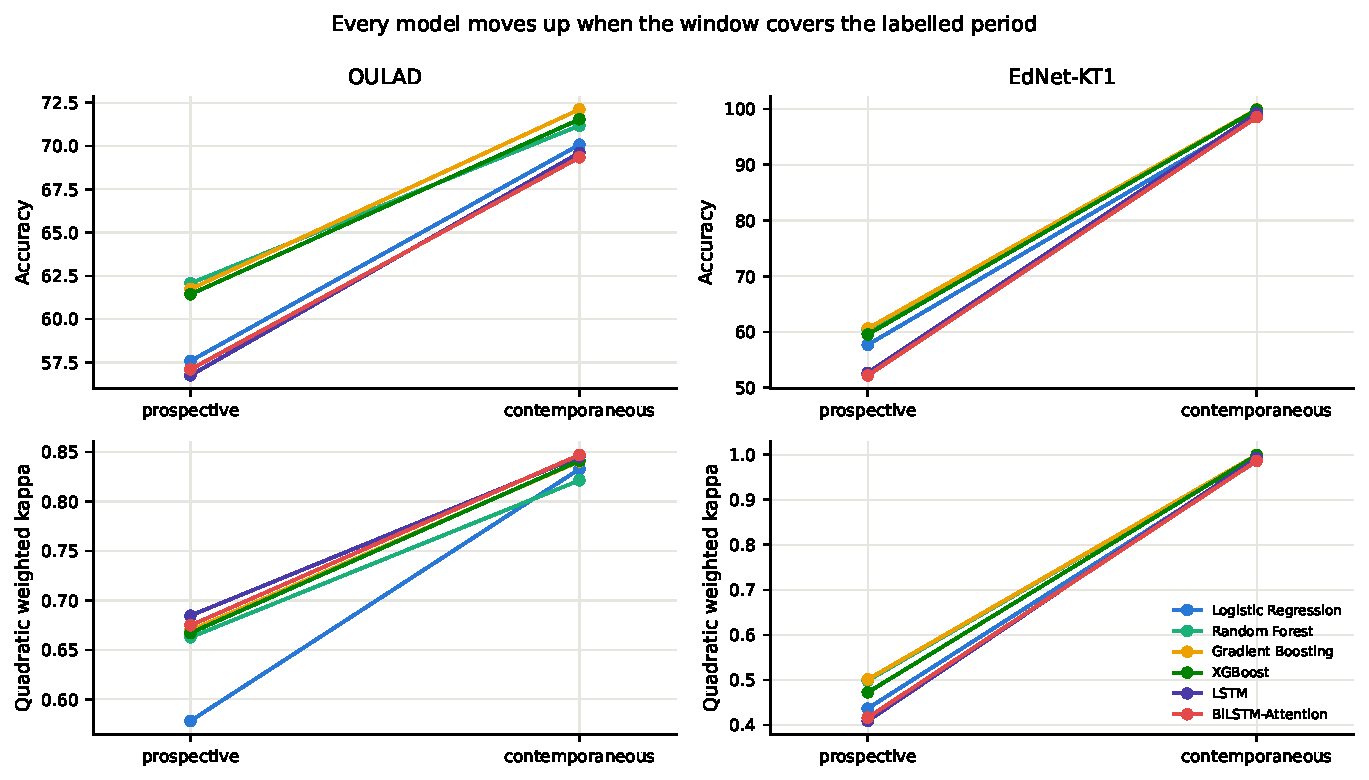
\includegraphics[width=0.95\textwidth]{figures/fig2_leakage_gap}
  \caption{The formulation effect by model and dataset: each line tracks one model from the prospective to the contemporaneous window. Every model moves up on both benchmarks; on EdNet-KT1 the movement approaches the reconstruction ceiling of a label that is a deterministic function of the full sequence.\label{fig:leakage}}
\end{figure}

\subsection{The Formulation Effect Is Graded: A Dose--Response Analysis}\label{sec:res_dose}

The two regimes of Section~\ref{sec:res_leakage} are endpoints of a continuum rather than a dichotomy. Figure~\ref{fig:dose} grows the OULAD feature window from the prospective cut ($p=0.30$) to the full course in four steps, holding target, student-level split, protocol, and models fixed; only the window moves. Reported performance rises \doseXGBmonotoneAcc{} with window share for every model: XGBoost accuracy climbs from \doseXGBaccFirst{} at the prospective cut to \doseXGBaccLast{} at the full window (QWK \doseXGBqwkFirst{} to \doseXGBqwkLast{}), and the recurrent models trace the same curve (BiLSTM-Attention QWK \doseLSTMqwkFirst{} to \doseLSTMqwkLast{}). Two readings follow. First, no threshold separates a ``safe'' window from a ``leaky'' one: growth up to $p{=}0.9$ reflects information that a later decision would legitimately acquire, while the final step adds the outcome-determining assessments --- only the matched-window control of Section~\ref{sec:res_decompose} attributes that last step to the label-defining signal itself. Window discipline is a matter of degree that must be disclosed, not a binary design choice. Second, the curve is a diagnostic for reading the literature: a score obtained under a partially overlapping window should be located on this curve rather than compared directly with either endpoint, and the \doseXGBaccLast{} full-window ceiling approaches, without exactly reaching, the contemporaneous configuration of Table~\ref{tab:leakage}, which additionally duplicates the full-window aggregates.

\begin{figure}[ht]
  \centering
  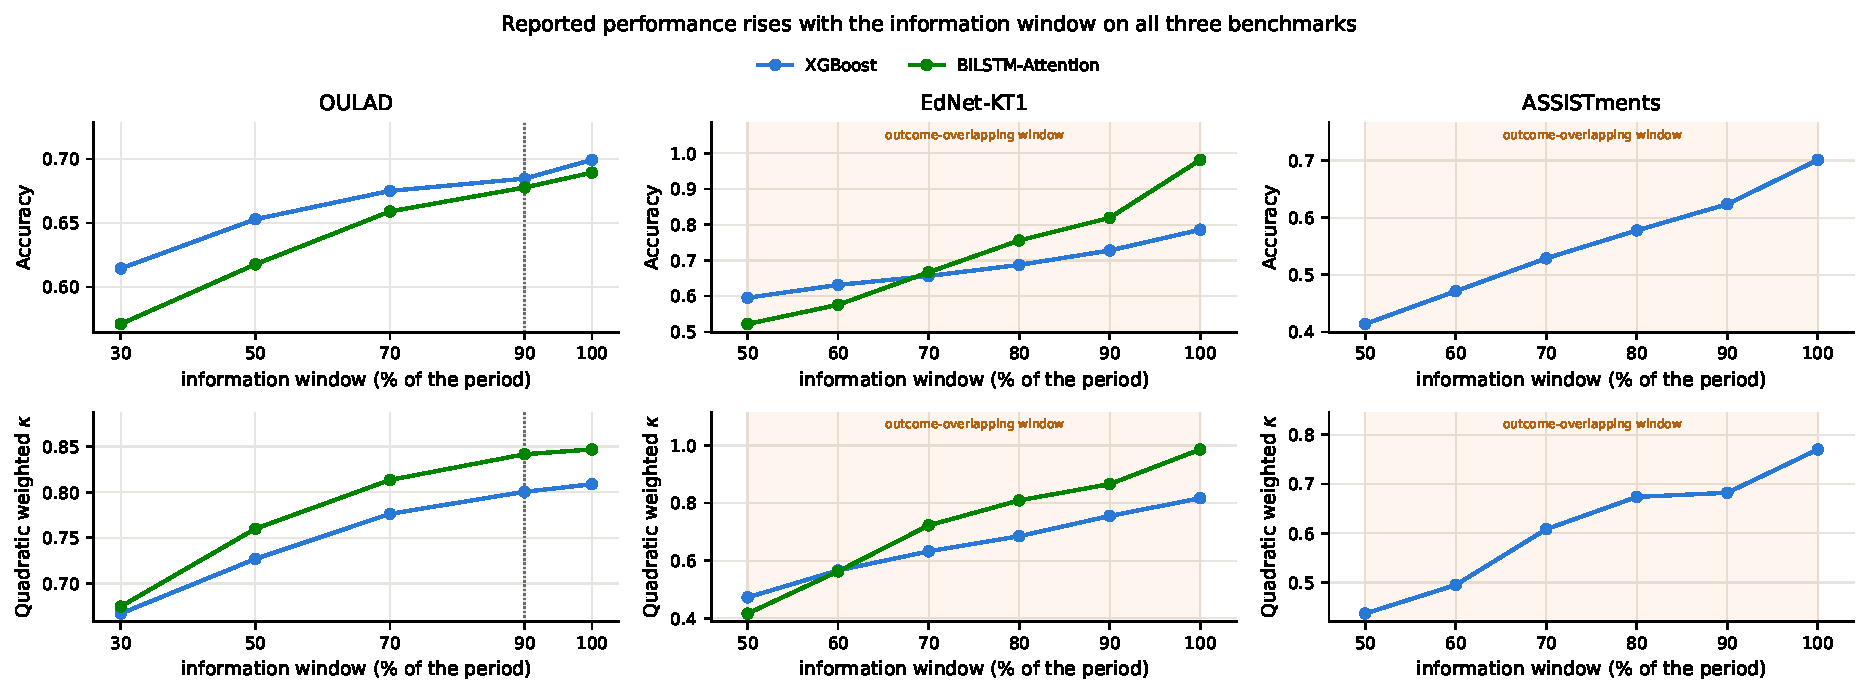
\includegraphics[width=0.95\textwidth]{figures/fig3_dose_response}
  \caption{The formulation effect is graded: accuracy (top) and quadratic weighted $\kappa$ (bottom) as the feature window grows on OULAD (left; dotted line marks the outcome-determining assessments) and EdNet-KT1 (right; shaded region is outcome-overlapping). Target, student-level split, protocol, and models are fixed; only the window share moves.\label{fig:dose}}
\end{figure}

The same dose--response on EdNet-KT1 (Table~\ref{tab:ednet_dose}) is steeper and ends at a different place. With the prospective label held fixed, accuracy climbs monotonically as the window invades the labelled period, reaching \ednetDoseXGBAcc{} for XGBoost and, strikingly, \ednetDoseBiAcc{} for BiLSTM-Attention at the full sequence --- essentially the reconstruction ceiling. Two aspects matter. First, the climb is smooth, confirming that contamination is graded rather than binary. Second, the recurrent model extracts the outcome-determining signal far more efficiently than the tree ensemble once it enters the window, which is precisely why EdNet-KT1 serves as the reconstruction-regime benchmark rather than as a realistic prediction task. The dose--response replicates on a third platform: on ASSISTments 2009--2010 (\assistCohort{} students; identical design), the tree ensemble climbs monotonically from \assistAccFirst{} to \assistAccLast{} (QWK \assistQwkFirst{} to \assistQwkLast{}). The recurrent model degenerated to majority-class prediction on this smallest cohort (its released results document the degeneration) --- sequence models, we note, require a scale that small institutional cohorts cannot supply.

\input{table_ednet_dose}

\subsection{Decomposing the Effect: Window Extension versus Label Leakage}\label{sec:res_decompose}

The formulation effect of Section~\ref{sec:res_leakage} mixes two components: information that legitimately arrives later in the course, and the label-defining signals that only exist once the outcome does. Table~\ref{tab:matched} separates them on OULAD by holding the window fixed and injecting exactly one label-defining variable --- the final-exam score. Two results stand out. First, the bulk of the effect is \emph{legitimate information accumulation}: extending the honest window from $p=0.3$ to $p=0.9$ --- every predictor recorded strictly before the outcome exists --- adds \matchedExtAcc{} accuracy points for XGBoost and \matchedExtAccBi{} points for BiLSTM-Attention (QWK $+\,$\matchedExtQwk{} and $+\,$\matchedExtQwkBi{}). Second, the injection itself contributes little at either window: at most \matchedLeakEarlyMax{} points at $p=0.3$ and \matchedLeakLateMax{} points at $p=0.9$ across all six models, because OULAD's outcome is only partly grade-determined --- withdrawal, its most severe class, is an administrative event rather than a function of marks (the residual distance to the full contemporaneous configuration of Table~\ref{tab:leakage} comes from its duplicated full-window aggregates). EdNet-KT1 fails in the opposite regime: its label is a deterministic function of the full sequence's correctness, so the contemporaneous regime reconstructs the label almost perfectly and essentially the whole gap is label leakage. Target leakage, in short, dominates when the label is grade-determined and is largely a red herring when it is not; in both cases the quantity that must be disclosed is the formulation effect --- the distance between the number a study reports and the number its decision time justifies.

\input{table_matched}

\begin{figure}[ht]
  \centering
  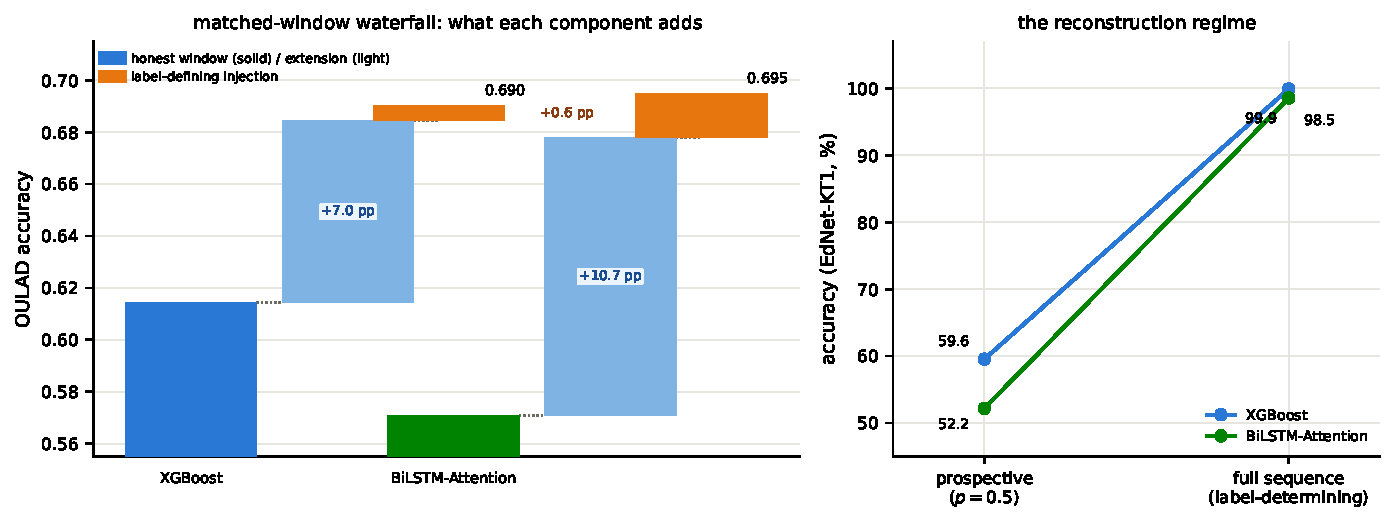
\includegraphics[width=0.95\textwidth]{figures/fig4_decomposition}
  \caption{Decomposing the formulation effect. Left: matched-window waterfall on OULAD --- extending the honest window from $p{=}0.3$ to $p{=}0.9$ (all predictors recorded before the outcome) contributes far more than injecting the label-defining final-exam score at the matched window. Right: on EdNet-KT1 the full sequence contains the outcome-determining signal by construction, and accuracy approaches the reconstruction ceiling.}
  \label{fig:decomp}
\end{figure}

\subsection{Generalization to a Future Cohort}\label{sec:res_temporal}

The random student-level split of Section~\ref{sec:protocol} mixes cohorts; a deployed system, by contrast, is always trained on the past and asked about the future. Table~\ref{tab:temporal} repeats the OULAD comparison under that deployment geometry: models are trained on the 2013 presentations only (students recurring in 2014 removed from training) and evaluated on the 2014 presentations. Absolute performance drops, as expected under a year of cohort drift --- prospective accuracy falls to \tempProsAccXGB{} for XGBoost (QWK \tempProsQwkLSTM{} for the LSTM) --- but the formulation effect survives intact: the contemporaneous window still buys \tempGapAccRange{} accuracy points and \tempGapQwkRange{} QWK across the three model families. The formulation effect therefore persists under a future-cohort evaluation that more closely approximates prospective deployment.

\input{table_temporal}

\begin{figure}[ht]
  \centering
  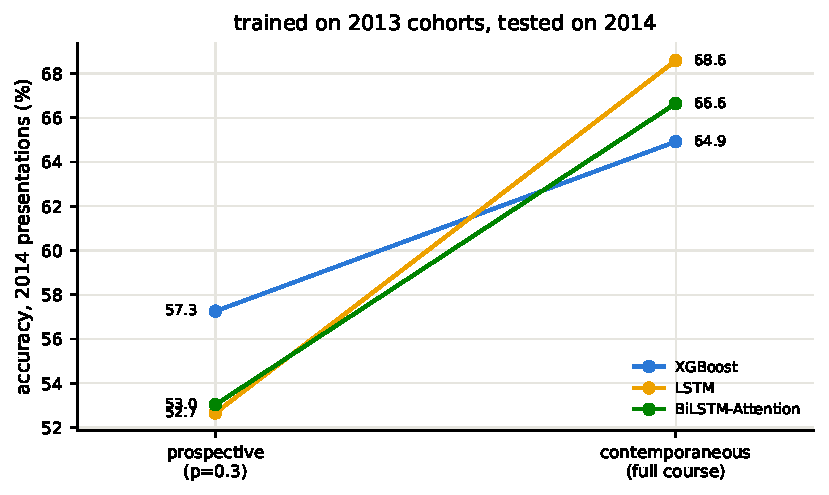
\includegraphics[width=0.7\textwidth]{figures/fig5_temporal}
  \caption{Future-cohort evaluation: accuracy of models trained on the 2013 presentations and evaluated on the 2014 presentations. The contemporaneous window raises every model, so the formulation effect is not an artifact of random resampling.}
  \label{fig:temporal}
\end{figure}

\subsection{Prospective Performance}\label{sec:res_prospective}

Tables~\ref{tab:oulad_prospective} and \ref{tab:ednet_prospective} report the full metric suite under the prospective protocol. No single family dominates. On OULAD the recurrent models achieve the best macro-F1 and QWK (LSTM \ouladProLSTMFone{}/\ouladProLSTMqwk{} against XGBoost's \ouladProXGBFone{}/\ouladProXGBqwk{}), while tree ensembles lead on accuracy; on EdNet-KT1 Gradient Boosting leads on accuracy and QWK, with the recurrent macro-F1 (\ednetProLSTMFone{}) inside its bootstrap interval. The family differences carry opposite significance on the two benchmarks: on OULAD the recurrent macro-F1 advantage is statistically clear (paired bootstrap over students, $p = \pOULADfam{}$ in favour of the LSTM), whereas on EdNet-KT1 the families are statistically indistinguishable in macro-F1 ($p = \pEdNetfam{}$) while Gradient Boosting retains the QWK lead. This is exactly why we report the trade-off family by family and metric by metric rather than claiming best-everywhere performance.

\input{table_oulad_prospective}

\input{table_ednet_prospective}

\begin{figure}[ht]
  \centering
  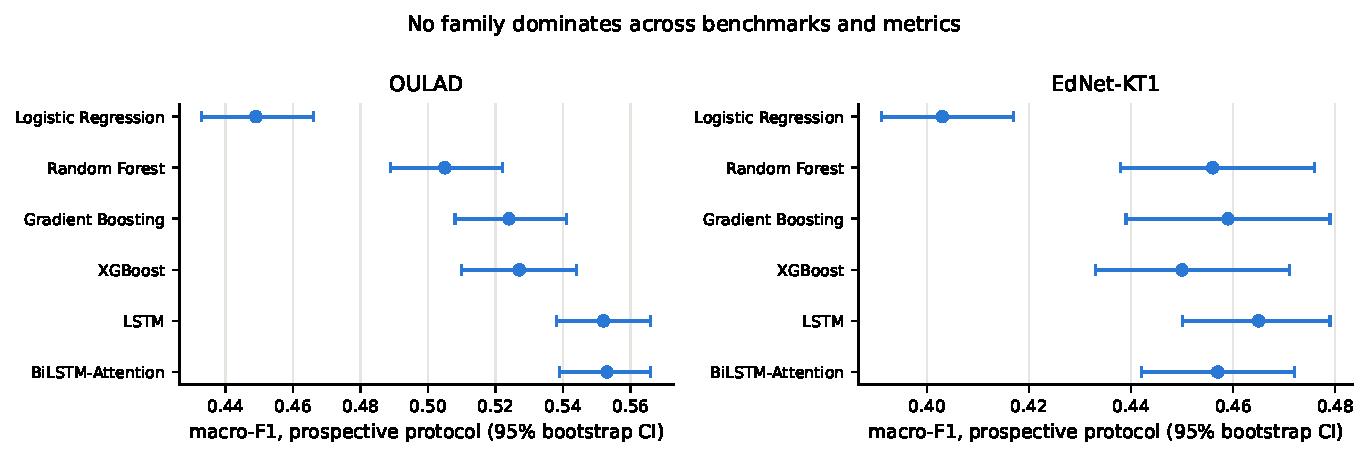
\includegraphics[width=0.95\textwidth]{figures/fig6_model_comparison}
  \caption{Prospective-protocol macro-F1 with student-level bootstrap 95\% intervals. No model family dominates across the two benchmarks; full intervals for every metric are released with the supplementary results.}
  \label{fig:modelcomp}
\end{figure}

\subsection{Ordinal Error Structure}\label{sec:res_ordinal}

Figure~\ref{fig:ordinal} decomposes prospective errors by ordinal distance. The bulk of prospective misclassifications fall on adjacent levels (one-level accuracy \ouladProXGBoff{} on OULAD, \ednetProBestoff{} on EdNet-KT1 for the best tree ensemble), but the severe-error columns of Tables~\ref{tab:oulad_prospective}--\ref{tab:ednet_prospective} must be read jointly, because the two model families fail in different directions. On EdNet-KT1 the class-weighted recurrent models allocate roughly a fifth of their predictions to the rare low levels and consequently record severe-underestimation rates of \ednetProLSTMsev{} (LSTM), whereas tree ensembles, which almost never predict below level~1, record only \ednetProBestsev{} (Gradient Boosting) --- at the price of the opposite error: \ednetProBestsevover{} of genuinely low-risk learners are flagged at levels 2--3 by the best tree ensemble, against \ednetProLSTMsevover{} for the LSTM. A classifier biased toward the majority levels minimises severe underestimation by construction, so neither rate alone ranks the families: underestimation measures missed interventions, overestimation measures false alarms, advisor load, and warning fatigue. On OULAD the asymmetry is smaller (best tree: \ouladProXGBsev{} under- versus \ouladProXGBsevover{} over-estimation). The contemporaneous regime suppresses exactly the underestimation column (Fig.~\ref{fig:ordinal}C), because the label-defining signals remove it; the apparent reliability of leaky systems is thus strongest precisely where a deployed system is most exposed. Confusion matrices (Fig.~\ref{fig:confusion}) localise the remaining mass.

\begin{figure}[ht]
  \centering
  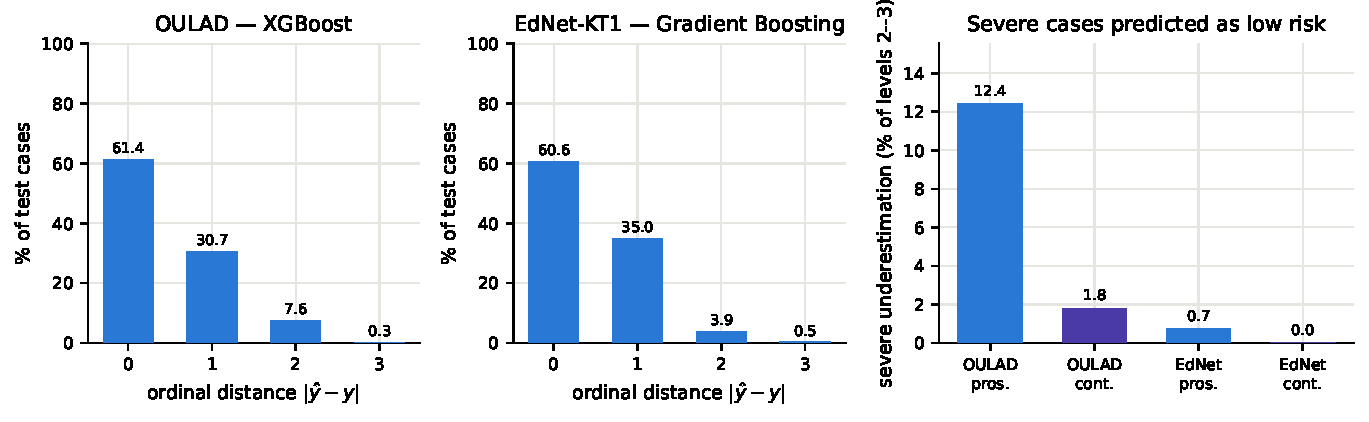
\includegraphics[width=0.95\textwidth]{figures/fig3_ordinal_structure}
  \caption{Ordinal error structure under the prospective protocol (best tree ensemble). Left: distribution of $|\hat{y}-y|$. Right: severe underestimation --- severe cases predicted as low risk --- as a fraction of level-2/3 cases.\label{fig:ordinal}}
\end{figure}

\begin{figure}[ht]
  \centering
  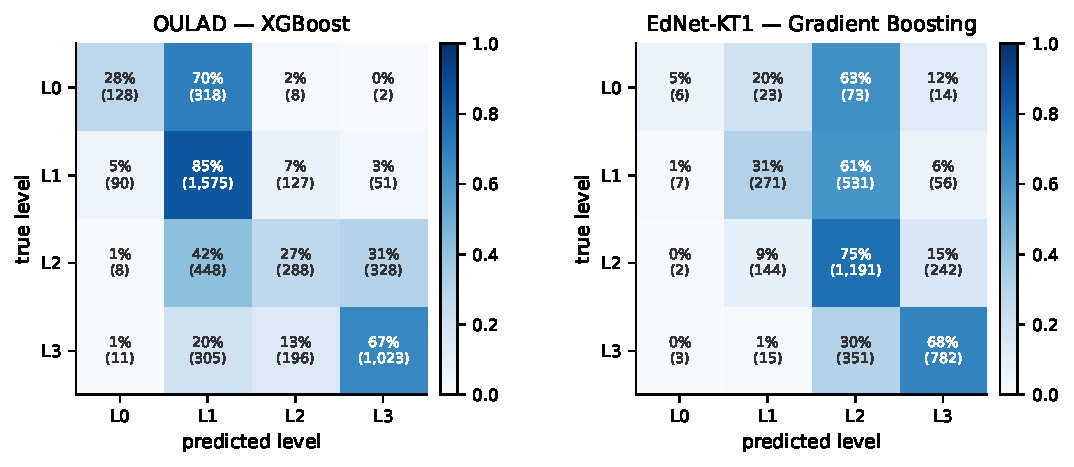
\includegraphics[width=0.95\textwidth]{figures/fig4_confusion}
  \caption{Confusion matrices under the prospective protocol (best tree ensemble per dataset).\label{fig:confusion}}
\end{figure}

\subsection{Attribution under the Corrected Protocol}\label{sec:res_shap}

Figure~\ref{fig:shap} ranks features by mean absolute SHAP value for the best tree ensemble on OULAD under the prospective protocol. Early assessment scores and early-window click aggregates dominate, followed by prior-study indicators; the profile is consistent with the regime in which the model operates --- everything ranked was observable at the cut-off by construction. Figure~\ref{fig:attention} shows the BiLSTM-Attention mean attention profile by predicted class: predictions of levels 0--2 concentrate their attention on the bins nearest the cut-off (34--43\% on the final bin), whereas predicted-severe (level 3) cases concentrate on the earliest bins (45\% on the first bin) --- a pattern consistent with the front-loaded, abruptly-stopped activity typical of withdrawal, reported strictly as a descriptive property of the model rather than evidence about student behaviour.

\begin{figure}[ht]
  \centering
  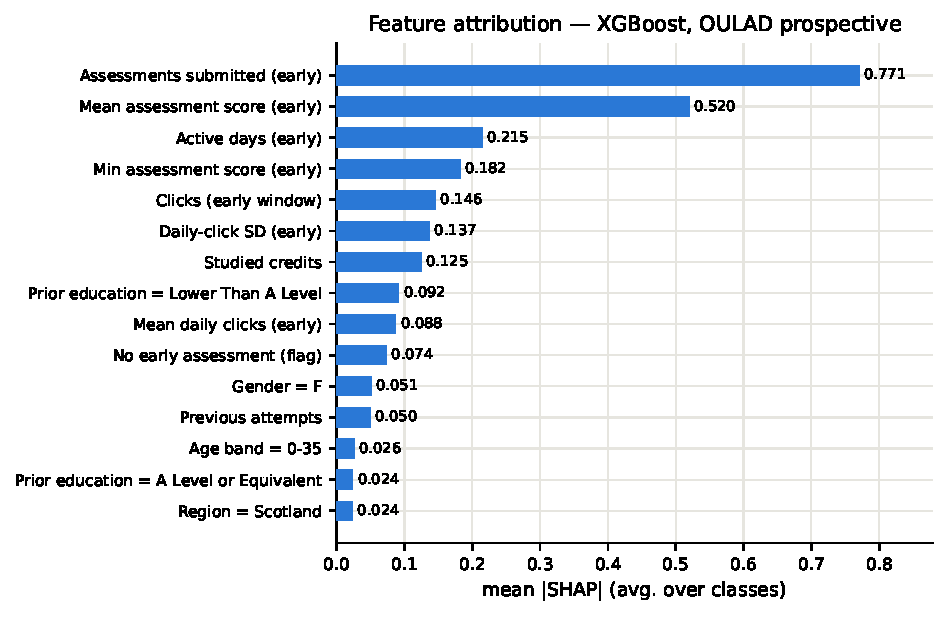
\includegraphics[width=0.9\textwidth]{figures/fig5_shap}
  \caption{Mean absolute SHAP values, best tree ensemble, OULAD prospective protocol. Higher values indicate features that contributed more to the model's output on average; the ranking is a property of the model, not a causal claim.\label{fig:shap}}
\end{figure}

\begin{figure}[ht]
  \centering
  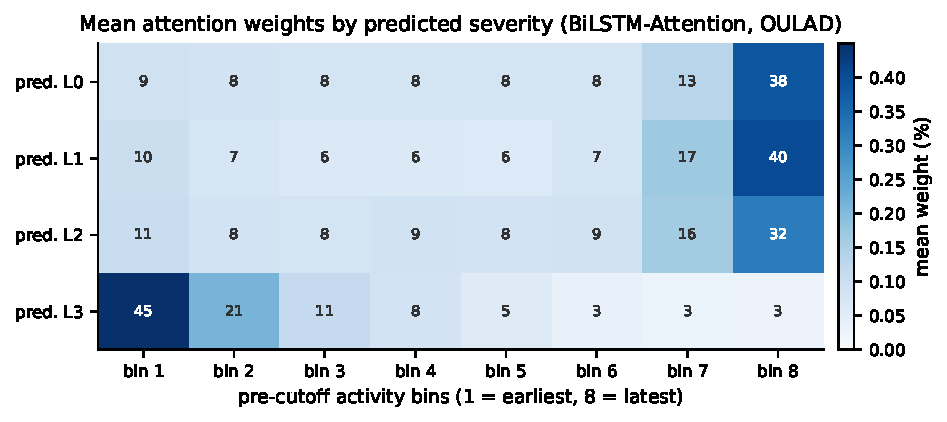
\includegraphics[width=0.85\textwidth]{figures/fig6_attention}
  \caption{Mean attention weights over the eight pre-cut-off activity bins, by predicted severity class (BiLSTM-Attention, OULAD prospective). Higher-severity predictions concentrate attention on the bins closest to the cut-off.\label{fig:attention}}
\end{figure}

%% =========================================================
\section{Discussion}\label{sec:discussion}

\subsection{What the Gap Means for Reported Results}\label{sec:disc_gap}

The measured gaps (\gapOULADaccRange{} accuracy points on OULAD; \gapEdNetaccRange{} on EdNet-KT1) are large enough to reorder a model comparison on their own. They also explain a familiar paradox: studies that adopt prospective windows and group-aware splits report modest numbers, while studies with outcome-window features report near-perfect ones. The 95\,\% student-level bootstrap intervals in Tables~\ref{tab:oulad_prospective}--\ref{tab:ednet_prospective} make a further point: under a clean protocol the uncertainty is non-trivial, and differences between strong models are often within a couple of points of each other's intervals --- unlike the formulation effect, which is far outside them. Formulation, not architecture, is the first-order variable.

\subsection{Practical Guidance}\label{sec:disc_guidance}

The protocol that produced these numbers reduces to the five rules of Table~\ref{tab:checklist}, all of which transfer directly to institutional analytics. The released pipeline implements rules R2 and R3 structurally rather than by convention: the prospective cut is enforced in the tensor constructor, not in the modelling script.

\begin{table}[ht]
\caption{A leakage-safety checklist for institutional risk-prediction studies. Each rule is enforceable in the data layer rather than by convention.\label{tab:checklist}}
\centering\footnotesize
\begin{tabular*}{\textwidth}{@{\extracolsep\fill}p{0.9cm}p{6.3cm}p{5.6cm}}
\toprule
\textbf{\#} & \textbf{Rule} & \textbf{Enforcement in this paper} \\
\midrule
R1 & Fix the operational decision time before writing down the model & cut-off $\tau$ stated per dataset (Table~\ref{tab:datasets}) \\
R2 & Restrict every predictor to information available at $\tau$; join label-defining variables at evaluation only & tensor constructor routes them to a post-cutoff table (Fig.~\ref{fig:pipeline}) \\
R3 & Split and resample at the student level & 70/15/15 by student; bootstrap resamples students \\
R4 & Fit every learned preprocessing step on training data only & imputation, encoding, scaling, class weights \\
R5 & Report ordinal error structure --- in particular severe under- and over-estimation --- next to accuracy & Tables~\ref{tab:oulad_prospective}--\ref{tab:ednet_prospective}, Fig.~\ref{fig:ordinal} \\
\bottomrule
\end{tabular*}
\end{table}

\subsection{Lessons from the Institutional Deployment Context}\label{sec:disc_deployment}

These rules were shaped by a two-year multi-source deployment in the vocational-college context that motivates this study, reported here as qualitative experience without institutional performance figures. Three lessons mattered most: workplace-learning variables contain legitimate structural zeros that naive imputation turns into false signals (hence the explicit zero-versus-missing flag); advisor-facing explanations saw adoption only once reduced to the three highest-magnitude attributions; and cross-system clock skew --- guarded by a differential-timestamp gate at the merge phase --- is the dominant reliability risk. None concerns model accuracy; all concern the data path that determines what a model can honestly be said to predict.

\subsection{Interpreting Attribution and Temporal Weights}\label{sec:disc_interpretation}

The SHAP and attention analyses should be read with their standard limits. Mean absolute SHAP values rank features by average contribution to this model's outputs under this protocol; they neither measure causal effects nor transfer automatically to other institutions whose label rules differ. Attention profiles describe where the recurrent encoder concentrated its mixture; they are evidence about the model, not about the student. For practitioners the value of profiles such as Fig.~\ref{fig:attention} is diagnostic rather than behavioural: a collapsed attention distribution would signal a model that ignores temporal structure, whereas the differentiated profiles confirm that the recurrent encoder exploits trajectory shape rather than only aggregated activity volume. We deliberately avoid causal phrasing in reporting both, and recommend the same discipline for applied learning-analytics work generally.

%% =========================================================
\section{Limitations}\label{sec:limitations}

Four limitations bound the conclusions. (1)~\emph{Label semantics.} Both benchmarks require mapping native outcomes onto an ordered scale; the OULAD mapping treats withdrawal as most severe. The formulation contrast --- the paper's target --- is invariant to any fixed relabelling shared by both regimes, and we verified this directly: re-running the full OULAD experiment under the alternative ordering that treats graded failure as most severe (Distinction $<$ Pass $<$ Withdrawn $<$ Fail) yields contemporaneous--prospective gaps of \ordAccRange{} accuracy points and \ordQwkRange{} in QWK, matching the primary ordering (\gapOULADaccRange{}; \gapOULADqwkRange{}). Absolute scores do shift with the ordering, so comparisons of the level scores themselves remain ordering-dependent. (2)~\emph{Dataset scope.} Experiments cover two public datasets; the institutional records that motivated the design cannot be released, so the institutional case appears only as software and qualitative experience. EdNet-KT1 results are computed on a large deterministic sample rather than the full corpus. (3)~\emph{Model scope.} Hyperparameters are fixed a priori and neural models are deliberately lightweight; the contemporaneous condition itself is an analytical stress test for measuring inflation, not a recommended prediction setting. As a robustness check, a post-hoc grid over hidden size ($\{32,64,128\}$) and learning rate ($\{3\times10^{-4},10^{-3},3\times10^{-3}\}$) for both recurrent models, selected on validation macro-F1 only, moved the best neural test macro-F1 on OULAD from \aprioriOULADFone{} to \tunedOULADFone{} (QWK \aprioriOULADqwk{} to \tunedOULADqwk{}) and on EdNet-KT1 from \aprioriEdNetFone{} to \tunedEdNetFone{} (QWK \aprioriEdNetqwk{} to \tunedEdNetqwk{}); the comparison of Section~\ref{sec:res_prospective} is unchanged, with tree ensembles retaining the QWK lead on EdNet-KT1 and the remaining macro-F1 differences falling inside the bootstrap intervals of Tables~\ref{tab:oulad_prospective}--\ref{tab:ednet_prospective}. Exhaustive tuning of every model could shift absolute numbers, but cannot affect the formulation effect the paper measures, because both regimes share the protocol. (4)~\emph{No intervention evidence.} Predictive performance is a prerequisite for, not evidence of, intervention effectiveness; estimating that requires controlled designs outside the scope of this paper.

%% =========================================================
\section{Conclusion}\label{sec:conclusion}

We measured what the outcome-window formulation is worth in academic risk prediction --- and, with a matched-window control, separated its label-defining component. Holding target, split, and protocol fixed, moving from a contemporaneous to a strictly prospective feature window costs \gapOULADaccRange{} accuracy points on OULAD and \gapEdNetaccRange{} on EdNet-KT1 across six model families, with ordinal agreement ($\kappa_w$) inflating by up to \gapOULADqwkMax{} and \gapEdNetqwkMax{} under the leaky formulation. Under the corrected protocol, lightweight temporal models are competitive but not dominant against tree ensembles when information access is held constant, and the residual error structure --- particularly severe underestimation of high-risk cases --- is the quantity that matters for deployment. We release the fusion pipeline, the experiment scripts, and every number-producing artefact so that the prospective formulation, not the contemporaneous one, becomes the default reporting standard for student risk prediction.

%% =========================================================
\bibliography{references}

%% =========================================================
\section*{Declarations}

\subsection*{Author Contributions}
J.H.\ and H.S.\ conceived the study and designed the research. J.H.\ developed the fusion pipeline, implemented the models and evaluation protocol, performed the experiments, prepared the figures and tables, and drafted the manuscript. X.D., W.S., and N.L.\ contributed to data curation, variable definitions, and validation of the educational context. J.S.\ contributed to institutional data-access coordination, project administration, and data-governance procedures. J.G.\ contributed computing resources and advised on the engineering implementation. H.S.\ supervised the study, revised the manuscript critically, and handled correspondence as the corresponding author. All authors reviewed and approved the final manuscript.

\subsection*{Conflict of Interest}
The authors declare no conflict of interest.

\subsection*{Data Availability}
All experiments in this paper use publicly available datasets. The Open University Learning Analytics Dataset (OULAD) \cite{Kuzilek2017} is available at \url{https://analyse.kmi.open.ac.uk/open_dataset} (CC BY 4.0). EdNet-KT1 \cite{Choi2020} is available at \url{https://github.com/riiid/ednet} (CC BY-NC 4.0). The ASSISTments 2009--2010 skill-builder dataset \cite{Feng2009} is available via its FigShare mirror (https://figshare.com/articles/dataset/skill\_builder\_data\_csv/25309000). No restricted institutional records were used in any experiment reported in this paper.

\subsection*{Code Availability}
The complete reproducibility package --- experiment scripts for both benchmarks, the evaluation protocol of Section~\ref{sec:protocol}, the student-level bootstrap, the attribution analyses, the figure-generation scripts, and the multi-source fusion pipeline with its synthetic-data harness --- is available at \url{https://github.com/Max-YUAN-22/prospective-risk-leakage} under the MIT licence. Every number, table, and figure in this paper is regenerated by the accompanying scripts from the public datasets; no reported value is manually transcribed.

\subsection*{Ethics Approval and Data Governance}
This study analyses two publicly released educational datasets under their respective licences, and reports qualitative experience from an institutional deployment conducted under the governance of Dongying Vocational College, which authorised secondary research use of fully anonymised administrative records; the corresponding author can provide the institutional authorisation documentation on request. No identifiable personal data were used at any stage: the institutional system is described at the level of software architecture and operational lessons only, and no institutional records or performance figures are reported.

\subsection*{Artificial Intelligence Declaration}
Artificial-intelligence tools were used for language editing and for assistance with drafting portions of the code and manuscript text under the authors' direction; the authors reviewed and take full responsibility for all content, and all experimental results were produced and verified by the authors' released scripts.

\subsection*{Funding}
This research received no specific grant from any funding agency in the public, commercial, or not-for-profit sectors.

\subsection*{Acknowledgements}
The authors thank the Open University (UK) and RIIID for making their datasets publicly available, and the Academic Affairs Office and Information Technology Center of Dongying Vocational College for supporting the deployment experience described in Section~\ref{sec:disc_deployment}.

%% =========================================================
%% End of manuscript
%% =========================================================

\end{document}
